This section provides a brief overview of further noteworthy tools and methodology I used throughout the refactoring process and in working with basf2 overall.

\subsubsection{OverlayFS}
OverlayFS \cite{overlayfs} is a Linux kernel file system that allows multiple directory layers to be combined into a single, unified view.
It achieves this by overlaying an upper directory (read-write) on top of a lower directory (typically read-only), presenting both layers as one merged file system at a specified mount point (see Fig.\ \ref{fig:overlayfs-schema} for a visualization).

When a file from the lower layer is modified, OverlayFS uses a copy-up mechanism: the file is first copied to the upper layer, and changes are applied there.
This ensures that the lower layer remains unaltered, while still allowing full read-write access through the upper layer.

During the V0Fitter refactoring process, I used OverlayFS to create a safe and flexible development environment by setting up overlay mounts for the basf2 repository and the software externals.
This approach was especially helpful in the early stages of my work, when I was still getting familiar with the framework and often introduced breaking changes.
With OverlayFS, I could easily return to a clean state by discarding the upper layer, significantly reducing the time required for environment recovery.

However, due to limited privileges on the shared Linux server used for development, I was restricted to using fuse-overlayfs \cite{fuse-overlayfs}, a user-space implementation with reduced performance compared to the kernel-mode OverlayFS.

Interestingly, I first learned about OverlayFS during a conversation with ChatGPT, when it recommended OverlayFS in response to my query for a method to efficiently mirror a directory in Linux in such a way that the original remained untouched.%
\footnote{\repoRef{chats/blob/main/v0fitter/questions/chatgpt/OverlayFS-Mirror-Setup.md}{chats/v0fitter/questions/chatgpt/OverlayFS-Mirror-Setup.md}}

\begin{figure}[h]
  \centering
  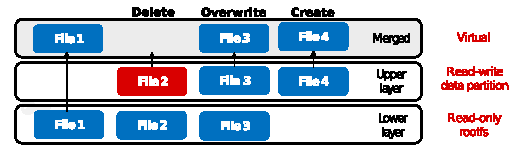
\includegraphics[width=0.7\textwidth]{static/overlayfs.pdf}
  \caption{Schematic: OverlayFS layered architecture and impact of file operations on directory layers \cite{overlayfs-schema}}
  \label{fig:overlayfs-schema}
\end{figure}

\subsubsection{VS Code GDB Debugging}
To decouple the UI from debugging backends, VS Code uses Debug Adapters that communicate with the UI via Microsoft's open-source Debug Adapter Protocol (DAP) \cite{dap}.
The editor's C/C++ extension \cite{vscode-cpptools} implements such adapters for multiple debuggers, notably the GNU debugger (GDB) \cite{gdb} on Linux.

Debugging a C/C++ binary involves defining a configuration in a launch.json file, where options such as setup commands for the debugger, program arguments, and environment variables can be specified.%
\footnote{For the launch.json file I used for basf2 debugging, see \repoRef{project/blob/main/artifacts/debugging.md}{project/artifacts/debugging.md}}
These setup commands for example allow to enable GDB's pretty-printing capabilities for C++ STL containers, resulting in improved display of objects like std::vectors in the debugging UI (see Fig.\ \ref{fig:vscode-debugging}, Left).

VS Code's debugging interface offers helpful features such as navigating between call stack frames and inspecting their variables in a side panel, while displaying the current execution position within the selected stack frame in the corresponding source file.
Additionally, both standard and conditional breakpoints can be set either through a dedicated panel or by clicking the area next to the source line number in the editor (Fig.\ \ref{fig:vscode-debugging}).

\begin{figure}[h]
  \centering
  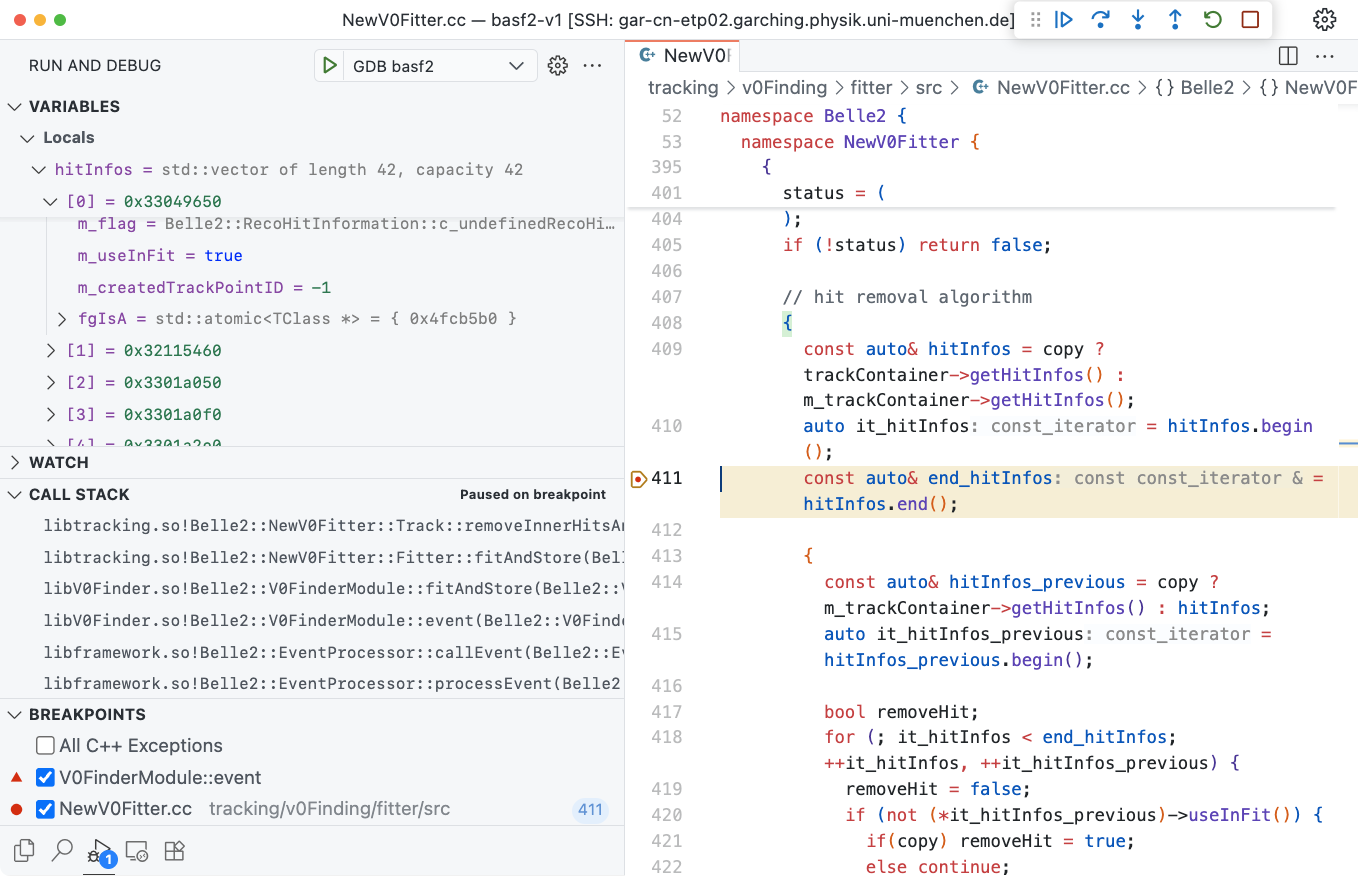
\includegraphics[width=0.9\textwidth]{static/vscode-debugging.png}
  \caption{Remote debugging of basf2 with VS Code and GDB\\%
    \emph{Left}: Debugging panel with variable, call stack and breakpoint inspector\\%
    \emph{Right}: Editor view with highlighted execution position and display of breakpoint locations
  }
  \label{fig:vscode-debugging}
\end{figure}

\subsubsection{V0Fitter debugging}
Using VS Codes debugging features, I was able to efficiently debug different V0Fitter implementations side-by-side, comparing their event handling.
To identify and analyze differences, I introduced event and track pair counters along with debug print statements into the module and fitter code.

Using vimdiff \cite{vim} to compare the log outputs from running v0ValidationGenerateSample with the different fitter versions then allowed me to pinpoint events with divergent behavior.
By subsequently setting conditional breakpoints using the counter variables' values, I could pause execution in both debugging sessions at the relevant positions, and step through processing in parallel.
It was through this process that I discovered that the primary reason for the NewV0Fitter's speed advantage was its strict invariant mass cut, which led to fewer track refitting calls.

VS Code's debugging capabilities also proved valuable for general debugging purposes during the development process.

\subsubsection{Clangd Extension}\label{sec:clangd}
The clangd extension for VS Code \cite{vscode-clangd} implements a client that communicates with clangd \cite{clangd}, a language server for C, C++ and Objective-C built on top of the Clang / LLVM compiler infrastructure.
By utilizing clangd's parsing, indexing and error analysis capabilities, the extension offers IDE-level functionality such as:
\begin{itemize}
  \item Navigation to symbol definitions across the entire codebase
  \item Inline display of compilation errors, warnings and static analysis results
  \item Display of type information, documentation and function signatures when hovering over symbols
  \item Project-wide symbol renaming functionality
  \item Auto-completion of symbol names and semantic code highlighting
  \item Inline annotation of types and function parameters (see gray code annot. in Fig.\ \ref{fig:vscode-debugging}, Right and Fig.\ \ref{fig:copilot-ui}, Left)
\end{itemize}
While the official VS Code C/C++ extension provides completion and analysis functionality as well, I found its engine to be less robust and performant, particularly for large projects, therefore I chose to disable this functionality in favor of clangd, while still using its debugging features as mentioned above.

To accurately parse all components of a project, clangd depends on a JSON compilation database, typically called compile\_commands.json. Most build systems can create these databases automatically during the build, for basf2 this is achieved by compiling with scons \mbox{{-}{-}create-json} <additional options>.

\subsubsection{Chat Exporting}
To document and compare GitHub Copilot's performance across different tasks, prompt formulations, and underlying LLMs, I needed a way to export AI interaction logs that were human-readable and information-rich.

The Copilot extension in VS Code provides limited export functionality, supporting only JSON format or manual copying of chat content in Markdown format.
Additionally, neither export method preserves model information, making later comparisons impossible.

To solve this problem, I developed a custom chat archiving utility that converts JSON chat logs exported from VS Code into annotated Markdown files.
The tool adds important metadata to the exported logs, especially the underlying model used for each response or code edit.
It also automatically generates diffs for any file changes made during a conversation.
All excerpts of Copilot chat logs and edit diffs shown in this section are from logs files generated using this chat archiver.
A brief implementation overview of the archiving utility is provided in Section \ref{sec:chat-archiver}.

For exporting ChatGPT conversations, I used ChatGPT Exporter \cite{chatgpt-exporter}, a browser script that supports single or bulk chat log exports in multiple formats.
I used its Markdown export feature to save notable ChatGPT conversations for documentation purposes.